\ChapterImageStar[cap:revisionLiteratura]{Revisión sistemática de la literatura}{./images/fondo.png}\label{cap:revisionLiteratura}

\mbox{}\\
\section{Construcción de la bitácora}

En búsqueda de una base teórica para la elección de una tecnología de virtualización basada en contenedores, 
se realizó una revisión del estado del arte. Esta revisión se completó en diferentes etapas:

\subsection{Planeación}

Esta etapa consistió en establecer el propósito general que se buscaba alcanzar con el \SMS\ (\textit{Systematic Mapping Study}). 
A su vez, definió aspectos como objetivos ver cuadro ~\ref{tab:metas}, preguntas de investigación ver cuadro~\ref{tab:preguntas} y métricas ver cuadro~\ref{tab:metricas}. Para ello, se siguió el modelo 
Objetivo-Pregunta-Métrica (\textit{Goal-Question-Metric}, GQM). A continuación, se definen los objetivos del \SMS\ aplicado 
a las tecnologías de virtualización basadas en contenedores en el cuadro.

\subsubsection{Definición de metas para el \SMS}

\begin{table}[H]
\centering
\renewcommand{\arraystretch}{1.2} % Espaciado reducido
\footnotesize % Texto más pequeño
\begin{tabular}{|c|p{13cm}|}  % Columna más ancha (12cm)
\hline
\textbf{Meta} & \textbf{Descripción} \\ \hline
G1 & Identificar trabajos con \VBC\ en docencia, investigación y extensión. \\ \hline
G2 & Clasificar trabajos con \VBC\ en dominios de \TI: desarrollo software, pensamiento computacional, computación paralela, análisis datos, IA, redes, infraestructura \TI, HPC, etc. \\ \hline
\end{tabular}
\caption{Definición de metas del SMS}
\label{tab:metas}
\end{table}

\subsubsection{Definición de preguntas de investigación}
\begin{table}[H]
\centering
\renewcommand{\arraystretch}{1.2} % Espaciado reducido
\scriptsize % Texto más pequeño
\begin{tabular}{|c|c|p{6cm}|p{6cm}|} % Columnas más estrechas
\hline
\textbf{Meta} & \textbf{Pregunta} & \textbf{Descripción} & \textbf{Motivación} \\ \hline

G1 & Q1 &
\textit{¿Cuáles trabajos con \VBC\ impactan positivamente en docencia, investigación y extensión?} &
\VBC\ ofrece transversalidad y reproducibilidad, facilitando transporte de soluciones TI entre dominios. \\ \hline

G2 & Q2 &
\textit{¿Cuáles trabajos con \VBC\ contribuyen en dominios de \TI?} &
Proporcionar base sólida para comprender estado del arte de \VBC\ sin análisis profundo. \\ \hline

\end{tabular}
\caption{Definición de preguntas de investigación del SMS}
\label{tab:preguntas}
\end{table}

\subsubsection{Definición de métricas}

\begin{table}[H]
\centering
\renewcommand{\arraystretch}{1.2} % Menor espaciado entre filas
\footnotesize % Texto más pequeño
\begin{tabular}{|c|p{9cm}|} % Columna de descripción más estrecha
\hline
\textbf{Métrica} & \textbf{Descripción} \\ \hline
M1 & Cantidad de trabajos identificados en cada dominio de \TI. \\ \hline
M2 & Cantidad de trabajos incluidos en educación. \\ \hline
M3 & Cantidad de trabajos incluidos en investigación. \\ \hline
M4 & Cantidad de trabajos incluidos en extensión. \\ \hline
\end{tabular}
\caption{Definición de métricas del SMS}
\label{tab:metricas}
\end{table}

\section{Búsqueda de estudios}

Esta etapa comprendió las siguientes secciones: 
\begin{enumerate}
  \item Estrategia de búsqueda, ya sea independiente o combinada;
  \item Identificación general de estudios;
  \item Revisión de estudios; y finalmente,
  \item Selección de estudios para incluir en el SMS.\@
\end{enumerate}

\subsection{Estrategia de búsqueda}

Este trabajo combinó las estrategias de búsqueda en bases de datos y búsqueda en bola de nieve. 
Para la estrategia de búsqueda en bases de datos, se seleccionaron las siguientes bases de datos: ACM, IEEE Xplore, Springer, Taylor \& Francis y Science Direct.

\subsection{Búsqueda en bases de datos}\label{subsec:busquedaBasesDatos}
Se seleccionaron las siguientes bases de datos para este propósito: ACM, IEEE Xplore, Springer, Taylor \& Francis y Science Direct.

\subsubsection{Identificación de estudios mediante búsqueda en bases de datos}\label{subsubsec:identificacionEstudios}
En esta etapa del proceso fue necesario establecer las palabras clave que serían útiles en las cadenas de búsqueda para cada una de las bases de datos seleccionadas. 
Los términos consideran los elementos identificados en la etapa de planificación, para lo cual también se utilizó el modelo PICOC ( \textit{Population}, \textit{Intervention}, \textit{Comparator}, \textit{Outcome}, and \textit{Context} ) como guía metodológica.

\begin{table}[H]
\centering
\renewcommand{\arraystretch}{1.2} % Espaciado reducido
\footnotesize % Texto más pequeño
\begin{tabularx}{\textwidth}{|p{0.18\textwidth}|X|} % Columna izquierda más estrecha
\hline
\textbf{Componente} & \textbf{Descripción} \\ \hline

Población & Trabajos sobre \VBC\ aplicadas en \TI, con énfasis en educación, investigación y extensión. \\ \hline

Intervención & Identificación y clasificación de trabajos \VBC\ en dominios de \TI. \\ \hline

Comparación & 
\textbf{1.} Comparación de proyectos \VBC\ por tasa de éxito en cada dominio \TI.\@        
\textbf{2.} Análisis de impacto de \VBC\ vs. otras soluciones en docencia, investigación y extensión. \\ \hline
Salida & Estructura de clasificación de trabajos \VBC\ que impactan en docencia, investigación y extensión. \\ \hline
Contexto & Docencia, investigación y extensión con apropiación de \VBC\ en \TI. \\ \hline
\end{tabularx}
\caption{Modelo PICOC}
\end{table}

\begin{table}[H]
\centering
\scriptsize
\setlength{\tabcolsep}{3pt}
\renewcommand{\arraystretch}{1.1}
\begin{tabular}{|p{3cm}|p{2.5cm}|p{2.5cm}|p{3cm}|p{3cm}|}
\hline
\textbf{Población} & \textbf{Intervención} & \textbf{Comparación} & \textbf{Salida} & \textbf{Contexto} \\
\hline
VBC \newline Dominios de \TI Educación Investigación Extensión & Identificación \newline Clasificación & Tasa de éxito \newline Evidencia de uso & Clasificación de trabajos \newline relacionados con VBC en cada dominio de \TI & Docencia Investigación Extensión \\
\hline
\end{tabular}
\caption{Palabras clave identificadas usando el modelo PICOC}
\label{tab:picoc}
\end{table}

\begin{table}[H]
\centering
\scriptsize
\setlength{\tabcolsep}{4pt}
\begin{tabular}{|p{5cm}|p{9.5cm}|}
\hline
\textbf{Palabras clave} & \textbf{Sinónimos} \\
\hline
Container-based virtualization & Application virtualization, Docker, Lightweight Virtualization \\
\hline
Education & Education System, Education Development, Higher Education \\
\hline
Research & Research Group, Research Proposal \\
\hline
Outreach & \IT\ Services, Technology Infrastructure, Cloud Computing \\
\hline
\end{tabular}
\caption{Palabras clave para la búsqueda en base de datos}
\label{tab:keywords}
\end{table}

\begin{table}[H]
\centering
\scriptsize
\setlength{\tabcolsep}{4pt}
\renewcommand{\arraystretch}{1.2}
\begin{tabular}{|p{4cm}|p{5cm}|p{5.5cm}|}
\hline
\textbf{Categoría} & \textbf{Inclusión} & \textbf{Exclusión} \\
\hline
Campos & Resumen & --- \\
\hline
Tipo de publicación & Artículos de revistas y conferencias & Tesis y capítulos de libros \\
\hline
Área/Disciplina & Management, \CS\, IT Management, engineering & Áreas no relacionadas con virtualización, \CS\ y \IT\ Management \\
\hline
Período & 2022 a 2024 & Antes de 2022 \\
\hline
Idioma & Inglés & --- \\
\hline
\end{tabular}
\caption{Criterios de Inclusión/Exclusión}\label{tab:criterios-inclusion-exclusion}
\end{table}

\subsubsection{Búsqueda en bases de datos}\label{par:busquedaBasesDatos}
Las cadenas de búsqueda se construyeron utilizando las palabras clave y sinónimos identificados en la tabla \ref{tab:keywords}.
Las cadenas de búsqueda específicas para cada base de datos se encuentran en~\ref{sec:cadenas-busqueda}.

\subsubsection{Resumen de la búsqueda en bases de datos sin criterios de inclusión/exclusión}\label{subsubsec:resumenBusqueda}
Este es el resultado antes de aplicar criterios de exclusión

\begin{table}[H]
    \centering
    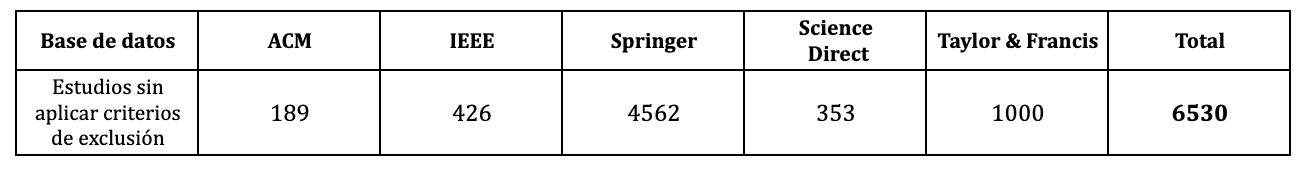
\includegraphics[width=\textwidth] {tablas-images/cp2/resumen-sin-criterios.png}
    \caption{Resumen de la búsqueda en bases de datos sin criterios de inclusión/exclusión}\label{tab:tabla-resumen-sin-criterios}
\end{table}
\begin{figure}[H]
    \centering
    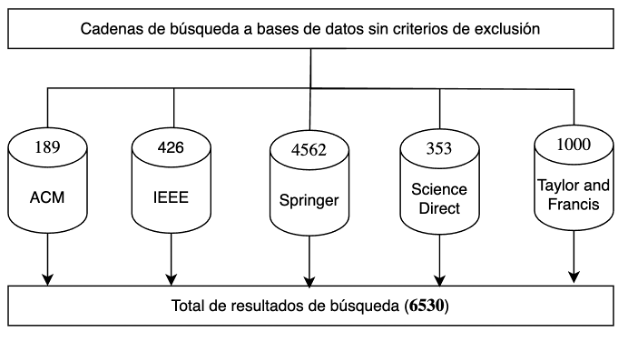
\includegraphics[scale=0.9]{tablas-images/cp2/bases-sin-criterio.png}
    \caption{Diagrama de búsqueda en bases de datos}\label{fig:tabla-resumen-busqueda}
\end{figure}

\subsubsection{Aplicación de criterios de exclusión de las bases de datos}
Esta búsqueda se realizó considerando los criterios de exclusión e inclusión definidos previamente.

Las cadena de búsqueda son exactamente iguales que antes, este punto se diferencia por la aplicación de 
filtros. Para ver las capturas de pantalla veáse el apéndice B sección 2.

\subsection{Resumen de la búsqueda en bases de datos con criterios de inclusión/exclusión}\label{subsec:resumenBusquedaCriterios}

\begin{table}[H]
\centering
\scriptsize
\setlength{\tabcolsep}{4pt}
\renewcommand{\arraystretch}{1.1}
\begin{tabular}{|l|c|c|c|c|c|c|}
\hline
\textbf{Bases de datos} & \textbf{ACM} & \textbf{IEEE} & \textbf{Springer} & \textbf{Science Direct} & \textbf{Taylor \& Francis} & \textbf{Total} \\
\hline
Con criterios aplicados & 48 & 134 & 592 & 46 & 156 & 976 \\
\hline
\end{tabular}
\caption{Resumen de la búsqueda en bases de datos con criterios de inclusión/exclusión}\label{tab:resumen-busqueda}
\end{table}
\begin{figure}[H]
    \centering
    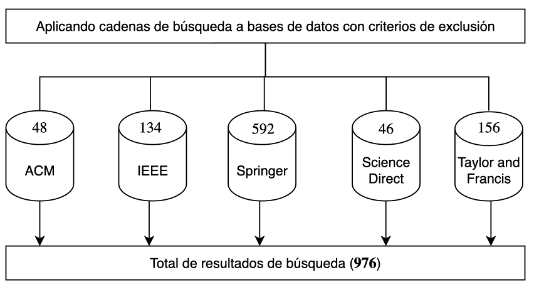
\includegraphics[width=\textwidth] {tablas-images/cp2/bases-con-criterio.png}
    \caption{Resumen de la búsqueda en bases de datos con criterios de inclusión/exclusión}\label{fig:tabla-resumen-busqueda-con-criterio}
\end{figure}

\section{Eliminación de duplicados}\label{sec:eliminacionDuplicados}
La eliminación de duplicados se realizó haciendo uso de la herramienta de gestión de referencias Mendeley. Luego de obtener los artículos se agregaron a Mendeley y esta herramienta se encargó de eliminar duplicados. En este punto se eliminaron 274 artículos duplicados.

\section{Priorización de estudios}\label{sec:priorizacionEstudios}

Luego de la selección inicial de los artículos, se procedió a revisar el \textit{title}, \textit{abstract} y \textit{keywords} de cada uno. Como resultado de esta revisión, se generaron métricas de calidad para cada artículo, con el fin de priorizar aquellos más relevantes para la investigación. Las métricas utilizadas fueron las siguientes:

\begin{itemize}
    \item \textbf{SCI} (Science Citation Index)
    \item \textbf{CVI} (Core Value Index)
    \item \textbf{IRRQ} (Index Relation Research Question)
\end{itemize}

Este proceso inició con un total de 771 artículos, los cuales fueron evaluados según su alineamiento con los objetivos de la investigación. La evaluación temática permitió identificar un total de 110 artículos con una relación directa con el enfoque planteado.

\section{Estrategia de búsqueda usando bola de nieve}\label{sec:bolaDeNieve}

En esta etapa, se seleccionó el primer cuartil según el índice \textbf{IRRQ}, lo que resultó en un total de 24 artículos. Adicionalmente, se incluyeron dos artículos por criterio de inclusión directa, estableciendo así una línea base de \textbf{26 artículos}. 

Sobre esta base, se aplicó la estrategia de \textit{bola de nieve} en ambas direcciones: hacia adelante y hacia atrás. Como resultado, se obtuvieron \textbf{87 artículos} mediante la técnica hacia atrás y \textbf{495 artículos} mediante la técnica hacia adelante. 

Esto definió un nuevo conjunto de artículos para un proceso de selección adicional (\textit{screening}). En esta fase, se eliminaron \textbf{14 duplicados} y \textbf{452 artículos} fueron descartados por no estar alineados con la investigación. 

Finalmente, se obtuvo un total de \textbf{116 artículos} mediante esta estrategia de búsqueda ampliada.

\section{Diagrama de búsqueda}\label{sec:diagramaBusqueda}

\subsection{Usando cadenas de búsqueda}
En el diagrama~\ref{tab:tabla-diagrama-cadena-busqueda} se puede apreciar la estrategia de búsqueda de artículos por medio de base de datos, aplicando las cadenas de búsqueda, se consolidaron los resultados de distintas bases de datos para obtener un total de 6530 resultados, posteriormente y aplicando criterios de exclusión se redujo esta cantidad a menos de 1000 resultados. Adicional a los criterios de exclusión, también se hizo eliminación de artículos duplicados, 205 por parte del ~\textit{Reference Manager} (Mendeley), y 69 por parte del ~\textit{SMS-Builder} para un total de 274 artículos removidos. Finalmente, se realiza la etapa de screening, donde se leen las secciones claves de los artículos, como ~\textit{abstract}, ~\textit{keywords} e introducción, a través de esto se pudo descargar 671 artículos que no eran pertinentes para el estudio.
\begin{table}[H]
    \centering
    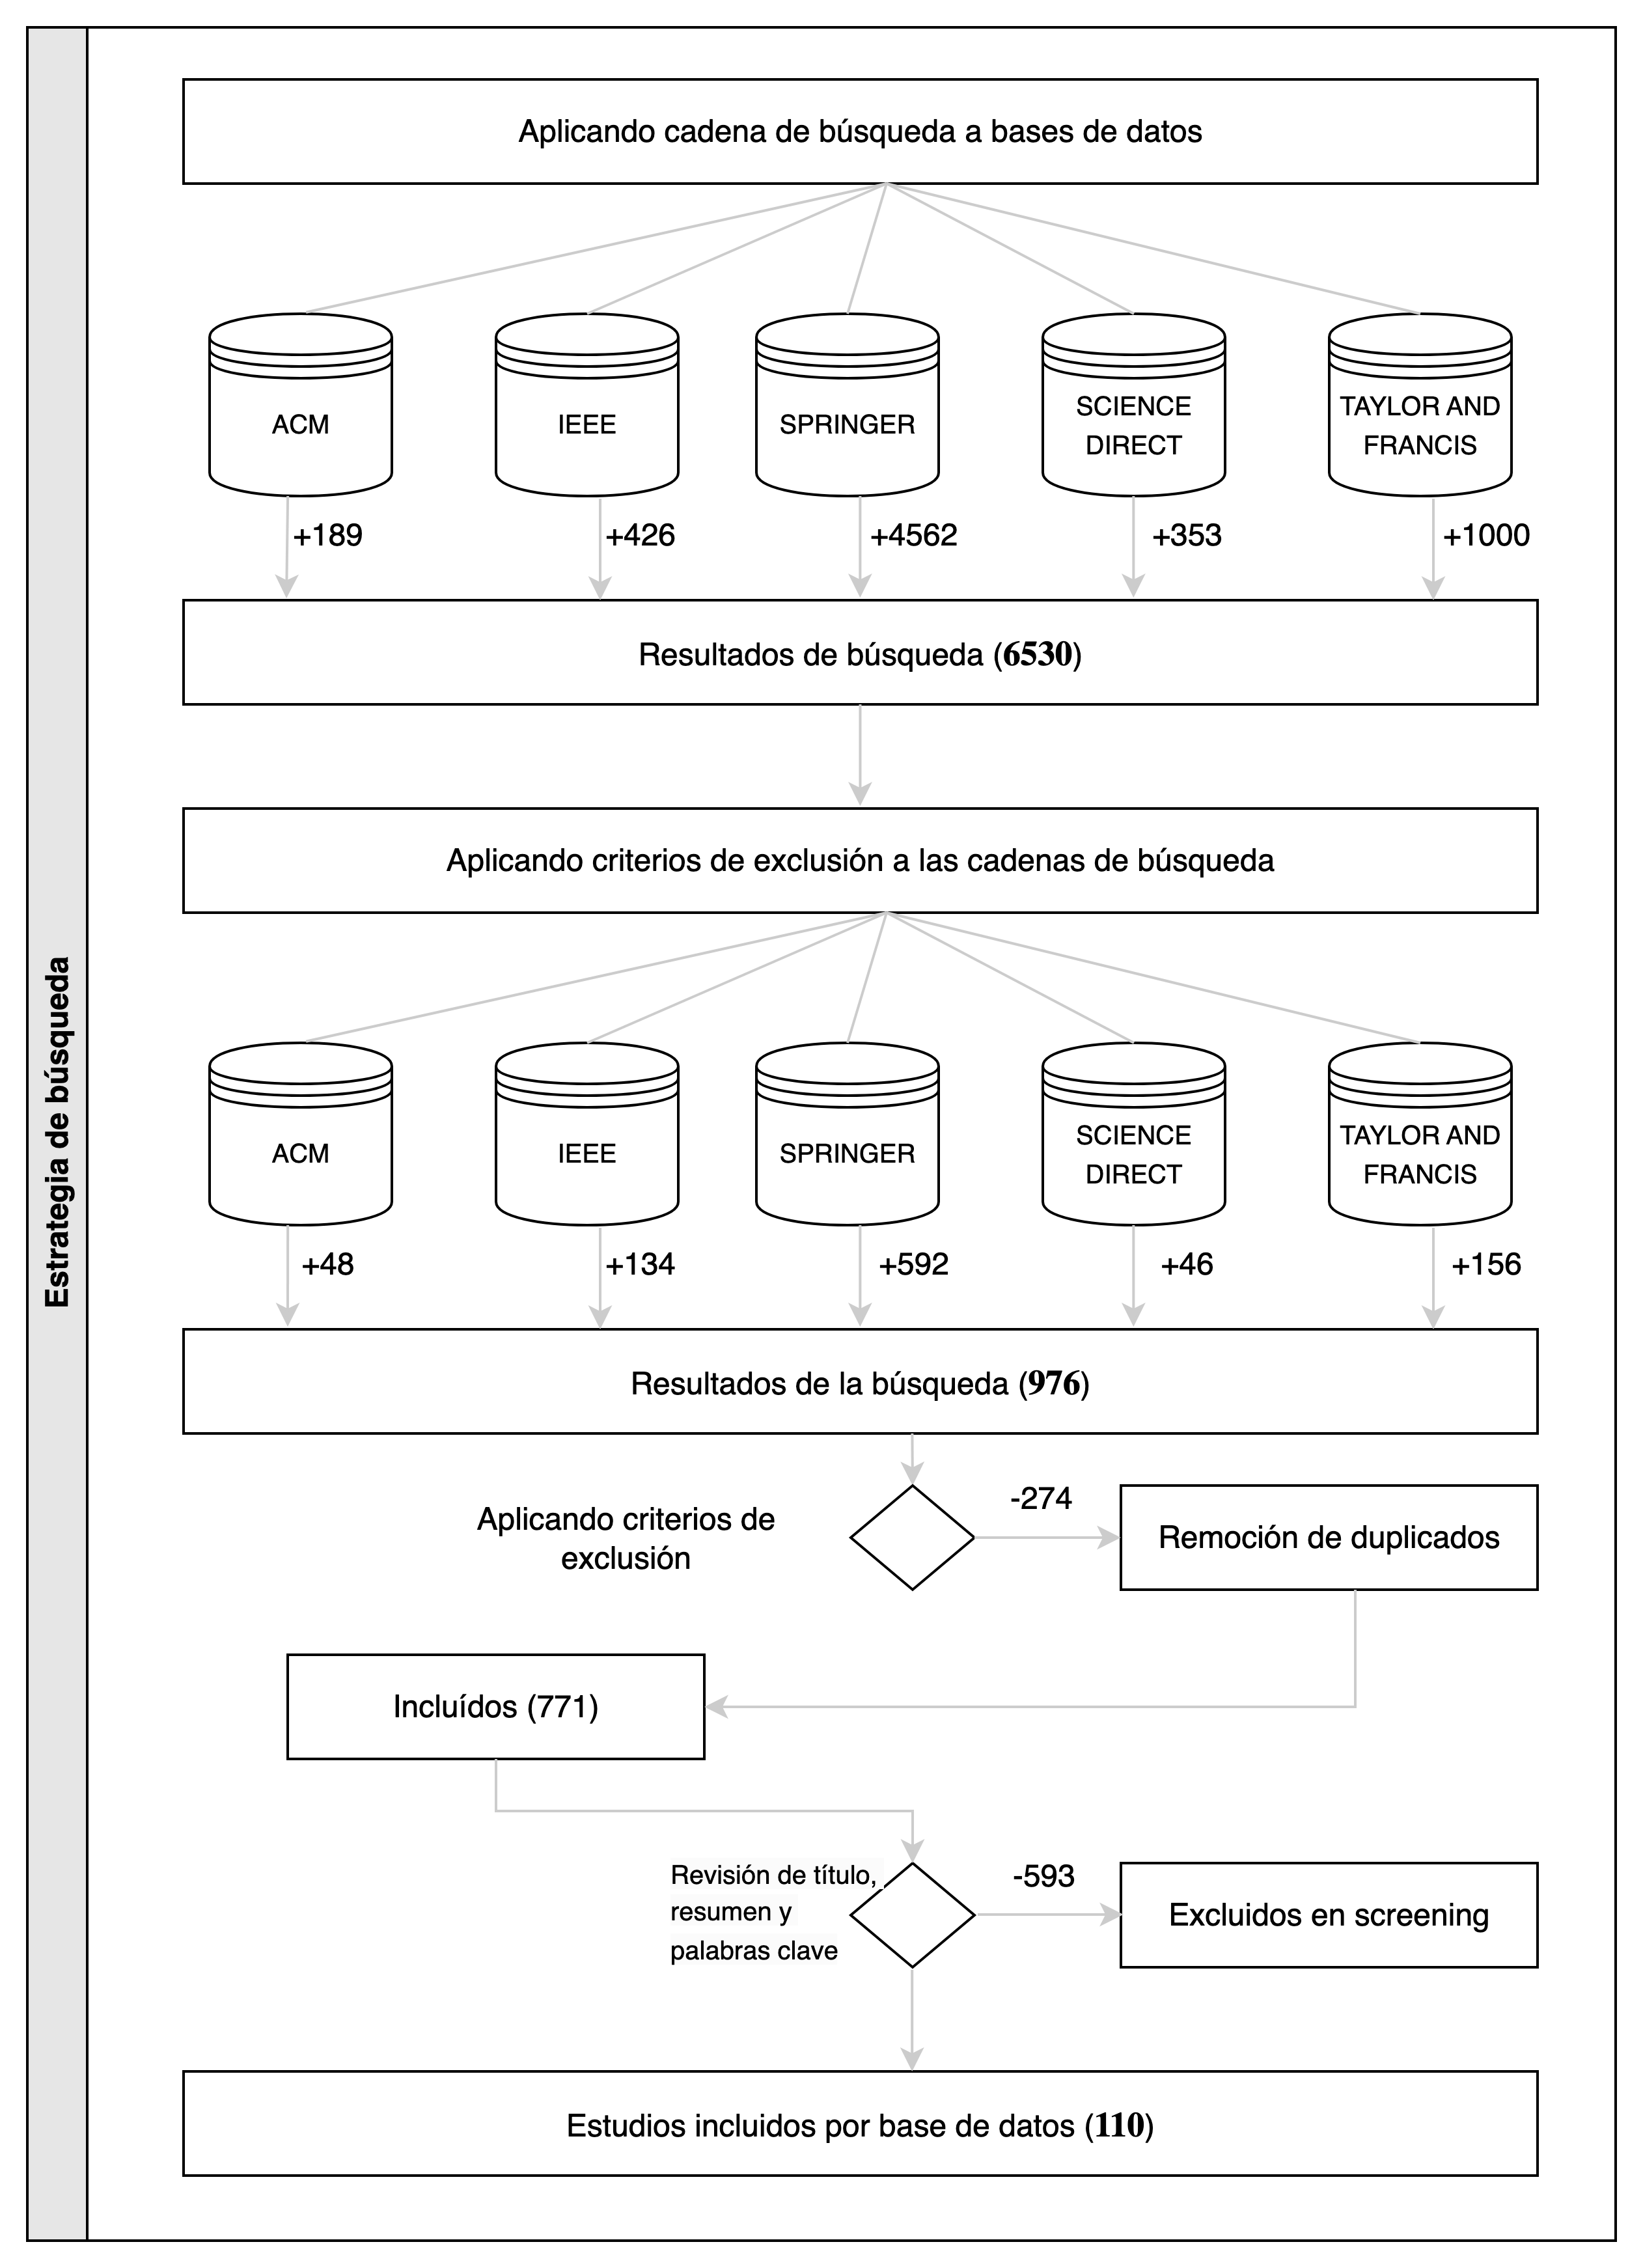
\includegraphics[scale=0.13]{tablas-images/cp2/diagrama-cadena-busqueda.png}
    \caption{Diagrama de la cadena de búsqueda}\label{tab:tabla-diagrama-cadena-busqueda}
\end{table}\label{img:busqueda-bd}

\subsection{Usando bola de nieve}
Como segunda estrategia de búsqueda dentro del SMS, se aplicó la técnica de ~\textit{Snowball}, la cual consiste en extraer artículos adicionales a partir de las referencias citadas en los estudios obtenidos en la estrategia anterior y de los estudios que citan a estos. De los 110 estudios del paso anterior, se seleccionan aquellos que tengan un SCI más relevante y se agrega uno por inclusión directa, con esto se obtiene un total de 25 artículos de línea base. Aplicando snowball hacia adelante (artículos referenciados) se obtienen 87 nuevos estudios, aplicando snowball hacia atrás (artículos que referencian el artículo base) se obtienen 495, para un total de 582. Finalmente, aplicando criterios de exclusión de remoción de duplicados y aplicando la técnica de screening, se obtiene un resultado de 116 artículos incluidos por bola de nieve. Todo este proceso se puede apreciar en la gráfica~\ref{tab:tabla-diagrama-bola-nieve-busqueda}.
\begin{table}[H]
    \centering
    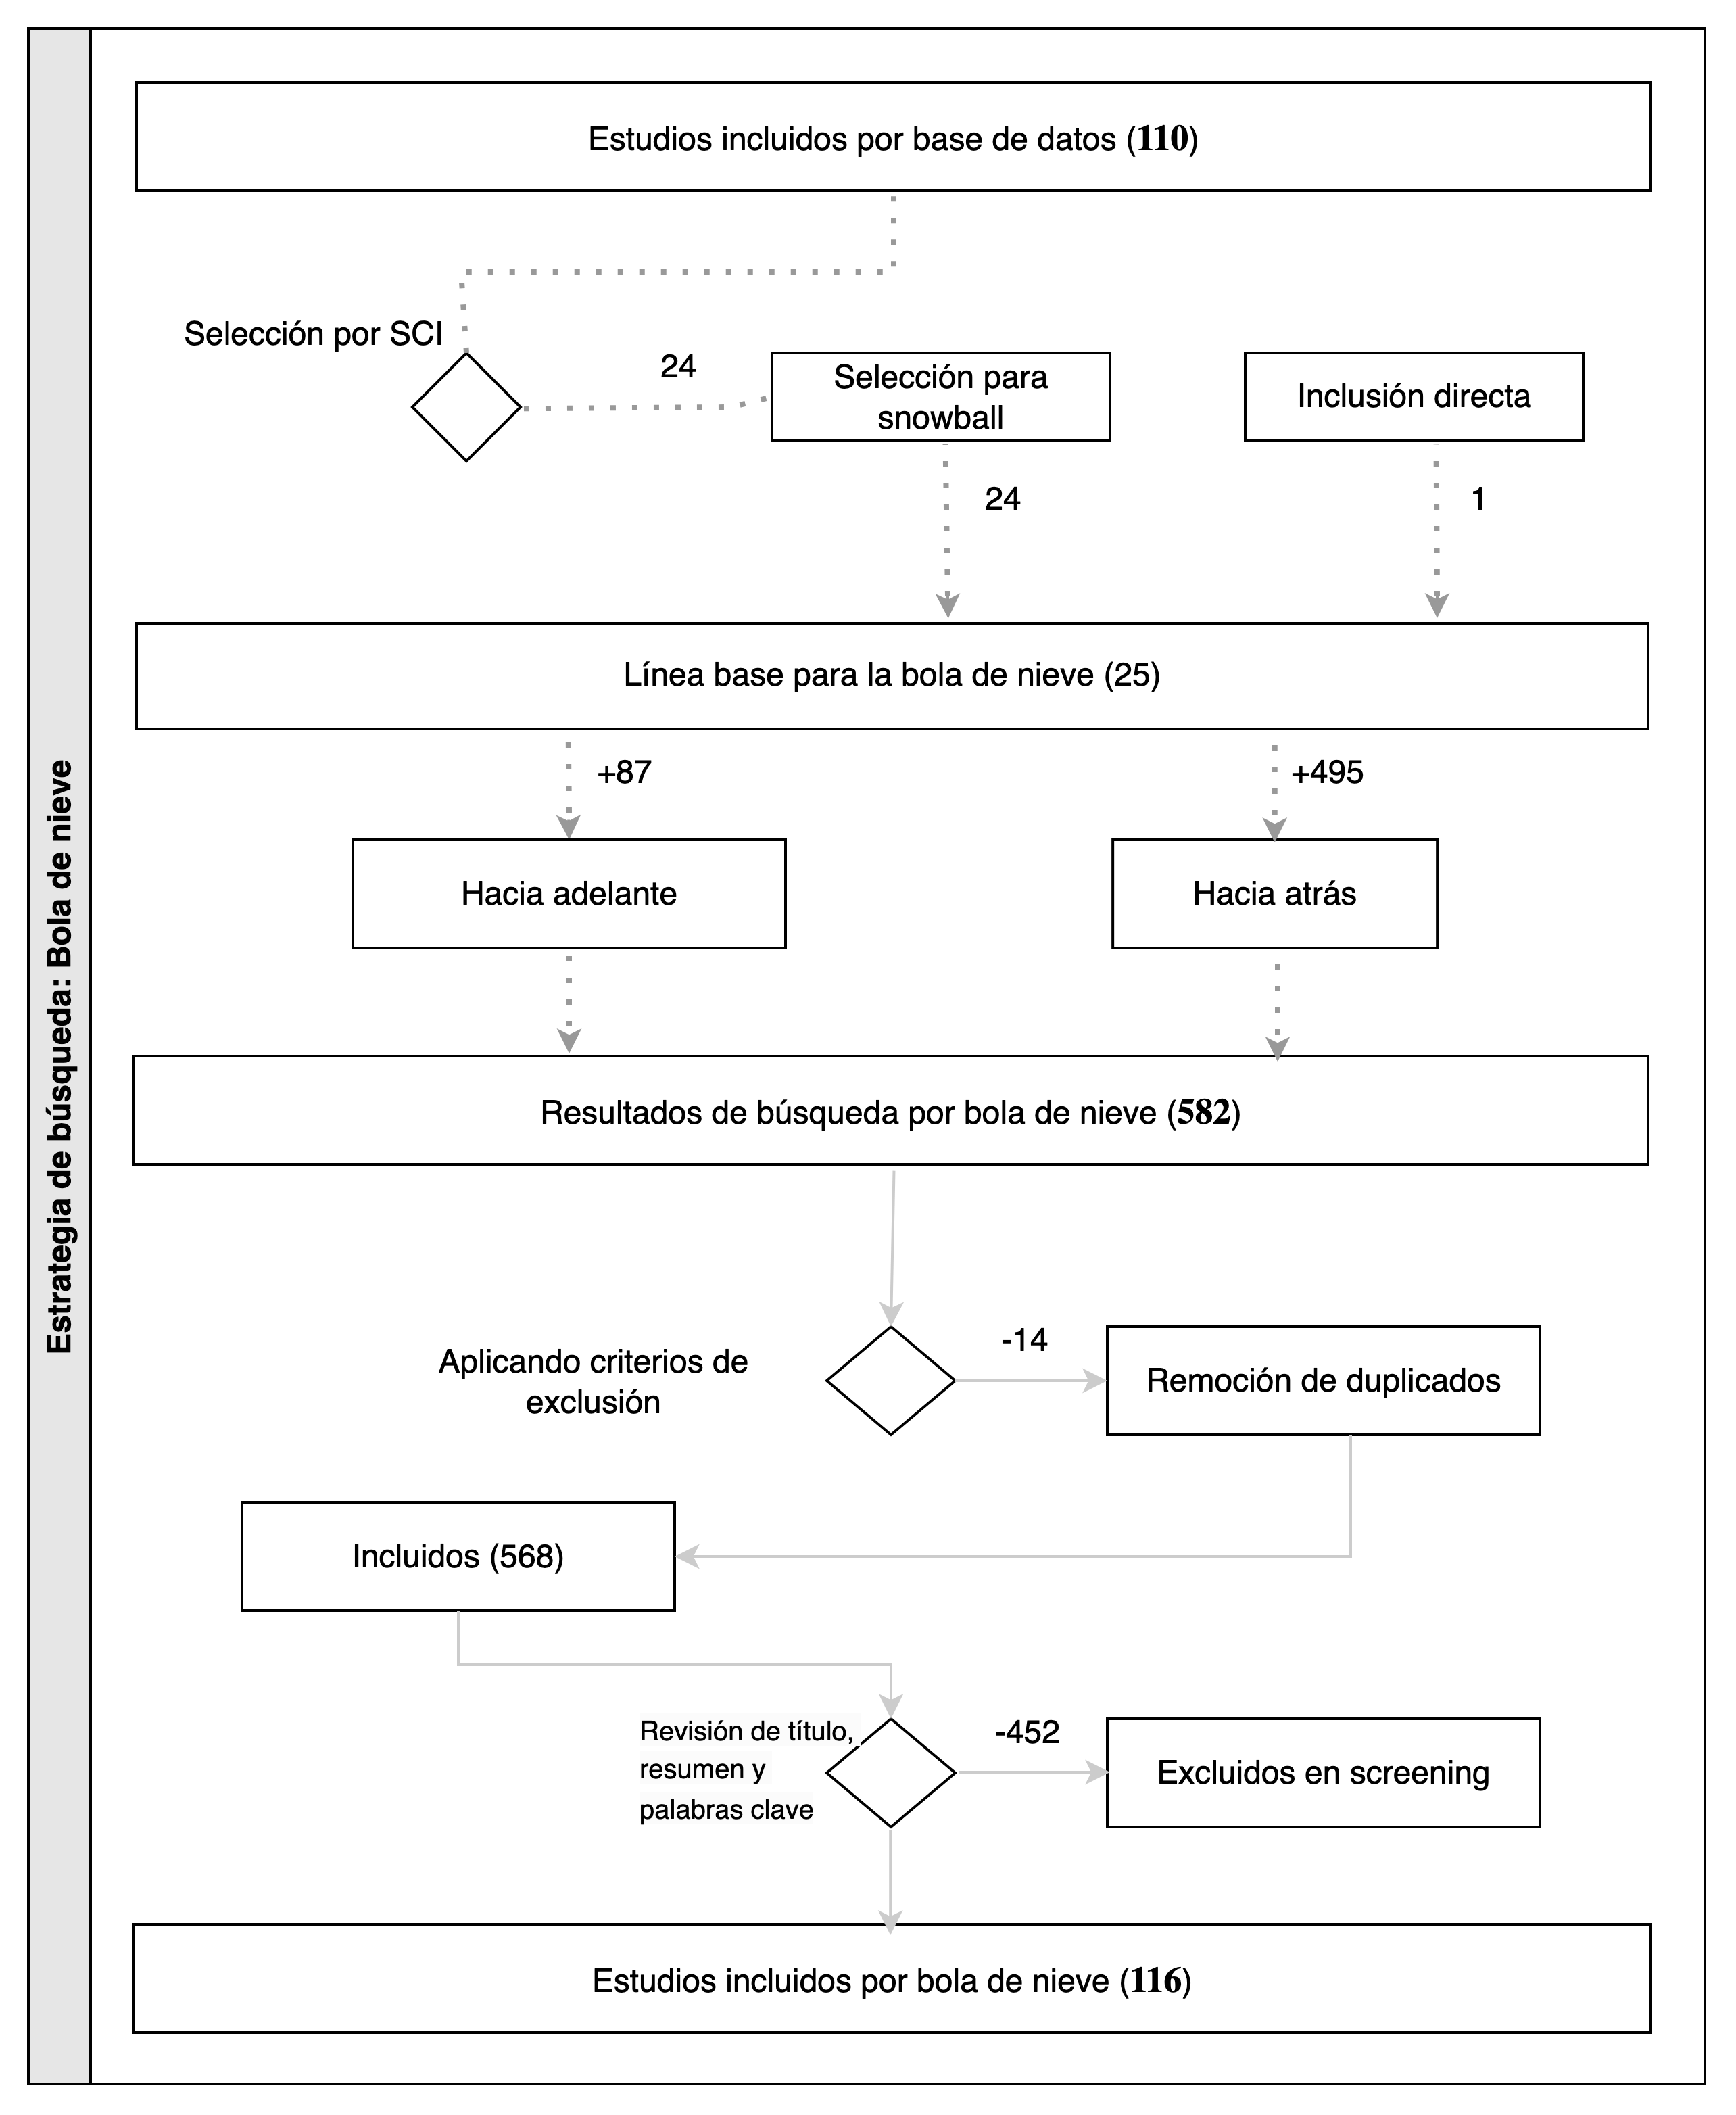
\includegraphics[scale=0.14]{tablas-images/cp2/diagrama-bola-nieve-busqueda.png}
    \caption{Diagrama de la búsqueda en bola de nieve}\label{tab:tabla-diagrama-bola-nieve-busqueda}
\end{table}

\section{Identificación de estudios}

\subsection{Artículos por año y métricas}
A continuación se presentan las gráficas que resumen los resultados de las estrategias anteriores. En la figura~\ref{fig:diagrama-articulos-ano-metrica} se pueden visualizar las métricas de calidad, separadas por los últimos 3 años y mostrando el promedio en cada métrica de los artículos publicados en esos años. En la figura~\ref{fig:tipos-articulos} se muestra el conteo de artículos por su tipo específico, el cual puede ser uno de 3 opciones: 'Revista', 'Conferencia' o 'Genérico'. Vemos que la mayoría de artículos provienen de revistas. En la figura~\ref{fig:estrategia-busqueda-articulos} se detalla la cantidad de artículos que se extrajo de cada estrategia. Finalmente, en la figura~\ref{fig:diagrama-red-articulos} se puede apreciar un diagrama de red, que segrega por colores los tópicos más relacionados entre sí
\begin{figure}[H]
    \centering
    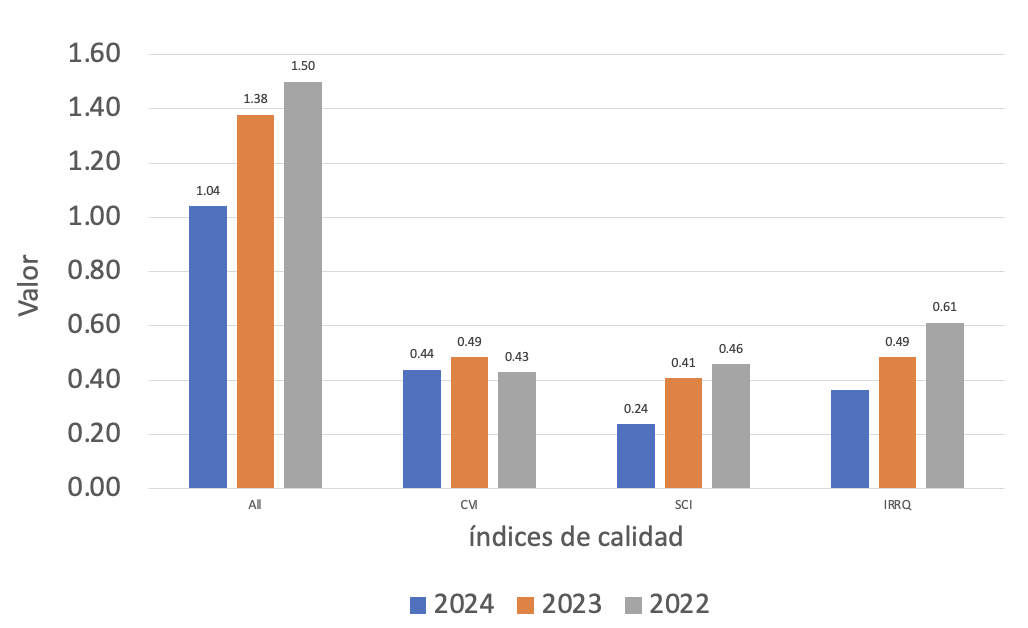
\includegraphics[width=\textwidth]{tablas-images/cp2/diagrama-articulos-ano-metrica.png}
    \caption{Artículos por métricas y año}\label{fig:diagrama-articulos-ano-metrica}
\end{figure}

\begin{figure}[H]
    \centering
    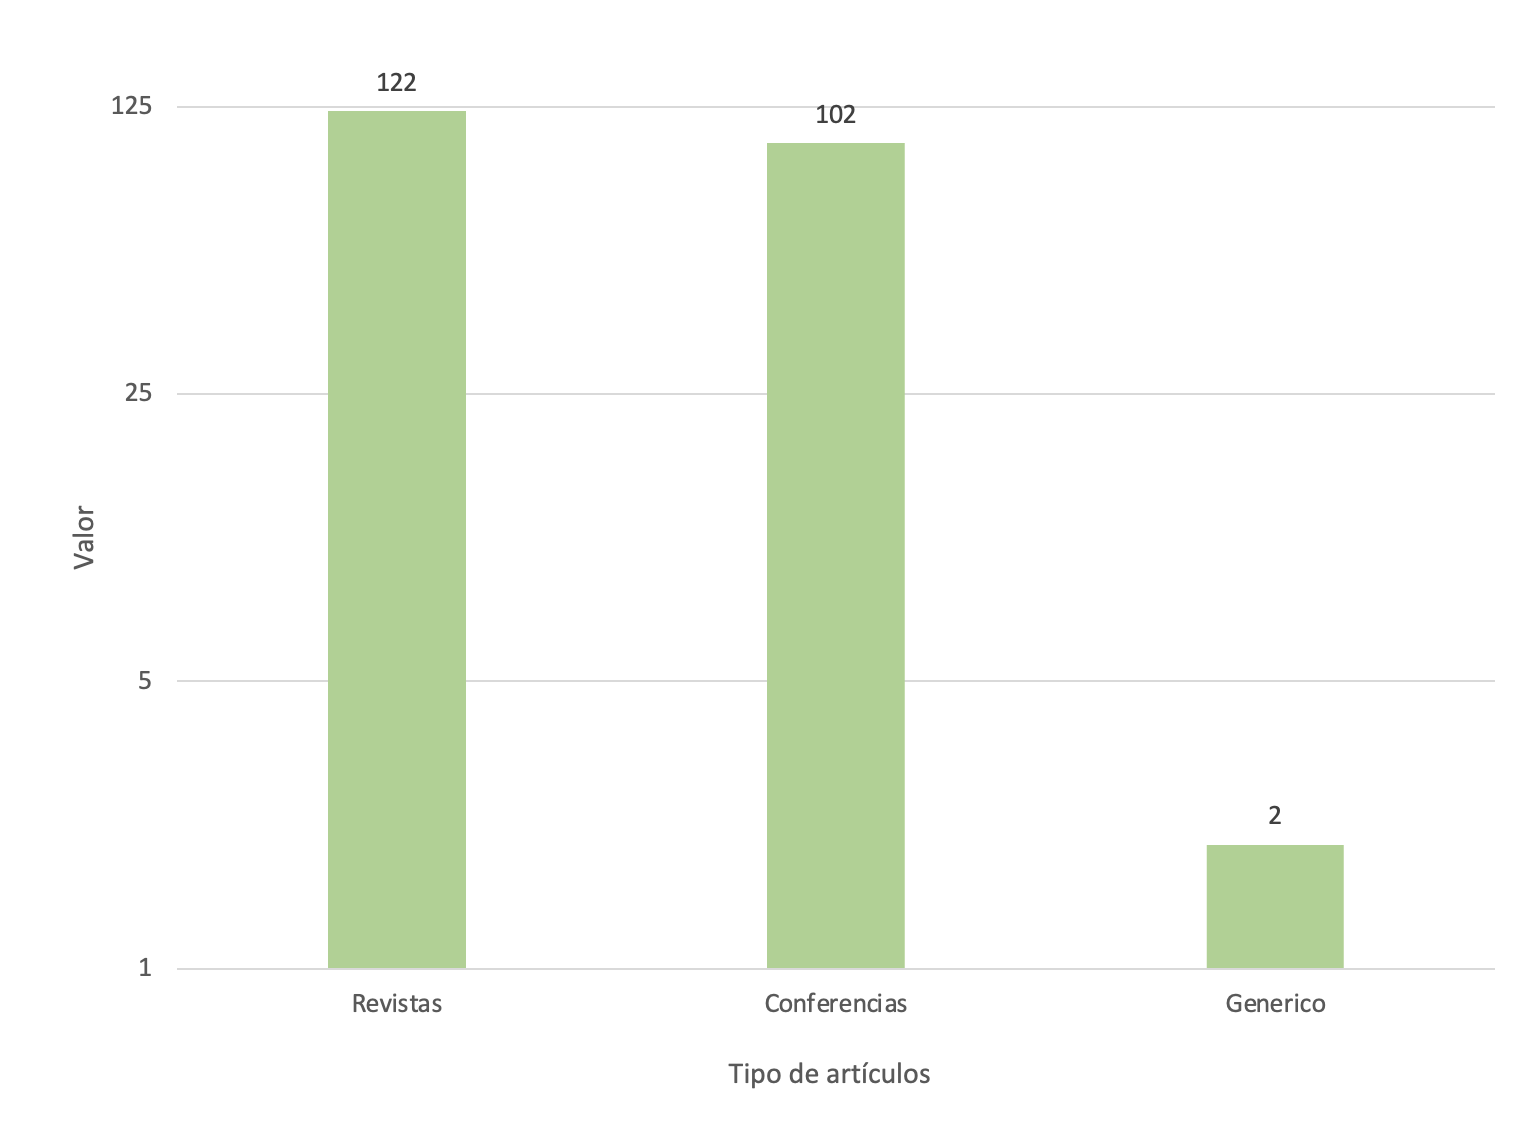
\includegraphics[width=\textwidth]{tablas-images/cp2/tipos-articulos.png}
    \caption{Artículos por tipo}\label{fig:tipos-articulos}
\end{figure}

\begin{figure}[H]
    \centering
    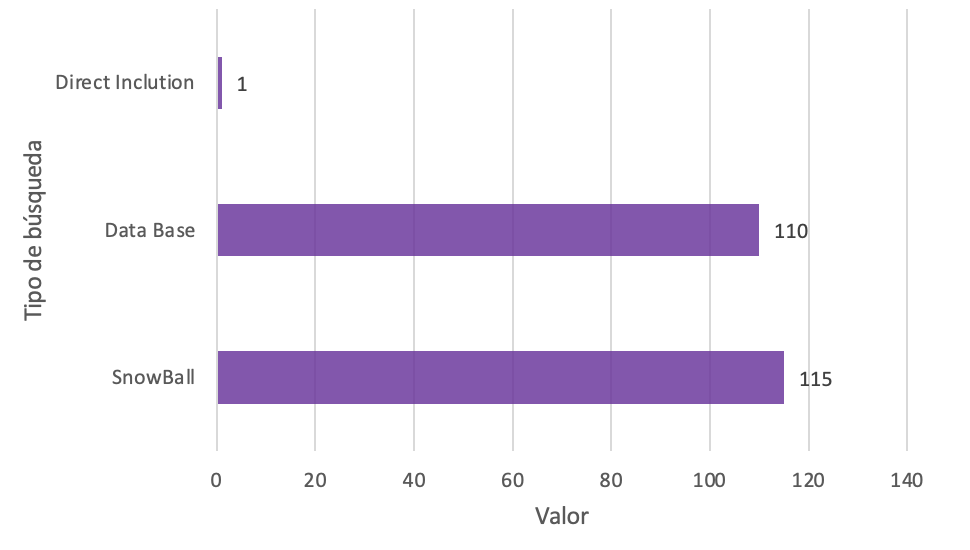
\includegraphics[width=\textwidth]{tablas-images/cp2/estrategia-busqueda-articulos.png}
    \caption{Estrategia de búsqueda de artículos}\label{fig:estrategia-busqueda-articulos}
\end{figure}

\begin{figure}[H]
    \centering
    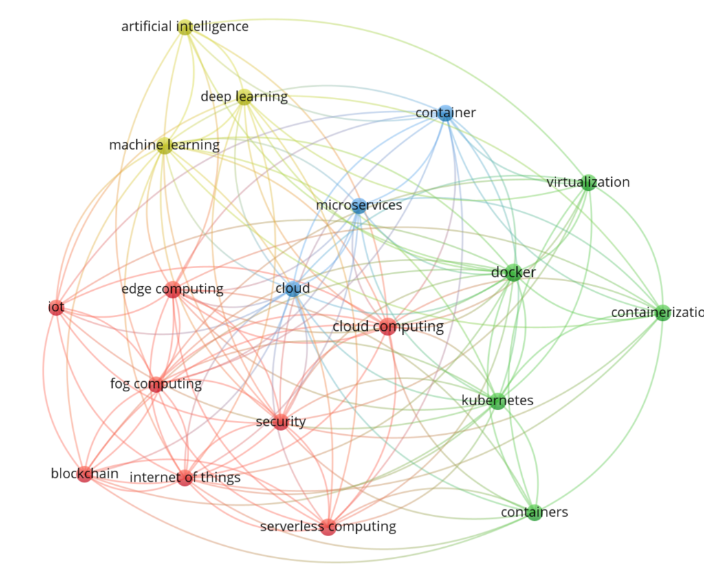
\includegraphics[width=\textwidth]{tablas-images/cp2/diagrama-red-busqueda.png}
    \caption{Diagrama de red de los artículos}\label{fig:diagrama-red-articulos}
\end{figure}

\section{Información de la herramienta}

\noindent
La herramienta utilizada para este proceso de revisión de la literatura fue \textbf{SMS-BUILDER}, la cual se encuentra disponible en \textit{Docker Hub}. El estudio realizado puede consultarse en el siguiente enlace:

\begin{center}
\href{https://sms-vbc.iti.grid.uniquindio.edu.co/}{\texttt{https://sms-vbc.iti.grid.uniquindio.edu.co/}}
\end{center}

\noindent
Adicionalmente, se implementaron procesos de respaldo como medida de seguridad. Estos \textit{backups} fueron almacenados en ubicaciones diferentes, siguiendo la estrategia de respaldo \textbf{3--2--1}.
